% !TEX program = xelatex
\documentclass[usenames,dvipsnames]{beamer}
\usefonttheme{serif}
\usefonttheme{structuresmallcapsserif}
\usetheme{Copenhagen}
\setbeamertemplate{headline}{} % This line removes the headline template
\usepackage{xcolor}
\beamertemplatenavigationsymbolsempty
\usepackage{tikz}
\usepackage{pgfplots}
\renewcommand{\qed}{\hfill\blacksquare}
\newcommand{\D}[1]{\Delta #1}
\renewcommand{\a}{\alpha}
\usepackage{float}
\setbeamertemplate{frametitle continuation}{%
    \ifnum\insertcontinuationcount>999999999 % this command tells the program when to start counting and also the count will be in numbers and not in roman letters
    \insertcontinuationcount
    \fi}
% ============================================================ %
% HEBREW support via polyglossia %
% ============================================================ %
\usepackage{polyglossia}
\defaultfontfeatures{Mapping=tex-text, Scale=MatchLowercase}
\setdefaultlanguage{hebrew}
\setotherlanguage{english}
\newfontfamily\hebrewfont[Script=Hebrew]{Arial}
% Use \begin{hebrew} block of text \end{hebrew} for paragraphs.
% Use \texthebrew{ } and \textenglish{ } for short texts.
% ============================================================ %
\title[]{{מאקרו א' - תרגול  7 - כלכלה בטווח הארוך}}
\author{\texthebrew{ מתן לבינטוב}}
\institute[{{ אב"ג}}]{{ אוניברסיטת בן גוריון בנגב}}
\date{}
\usepackage{bidi}
\begin{document}
\begin{RTL}
\begin{frame}
\titlepage
\end{frame}
\begin{frame}
    \frametitle{נושאים}
    \tableofcontents
    

\end{frame}
\section{הנחות}
\begin{frame}[allowframebreaks]
    \frametitle{הנחות}
    קיימים 3 גורמי יצור הקובעים את כושר היצור של המשק: 
    \begin{enumerate}
        \item $L$ - כוח העבודה
        \item $K$ - מלאי ההון
        \item $A$ - רמת הטכנלוגיה
    \end{enumerate}

    \begin{block}{פונקציית היצור}
        $$Y = AF(K,L)$$
    \end{block}
    \begin{block}{הנחות}
        \begin{itemize}
            \item בטווח ארוך גורמי היצור קבועים ולכן התוצר גם קבוע - $\bar Y = \bar A F(\bar K, \bar L)$
            \item תפוקה שולית חיובית - $F_K = MPK > 0 , F_L = MPL > 0$
            \item תפוקה שולית פוחתת - $F_{KK} < 0 , F_{LL} < 0$
            \item תק''ל - תשואה קבועה לגודל
        \end{itemize}
    \end{block}
    \end{frame}

    \begin{frame}
        \frametitle{גרף יפה}
        \begin{center}
        \begin{tikzpicture}
            \begin{axis}[
                xlabel={$K$},
                ylabel={$Y$},
                axis lines=left,
                ymax=10,
                ymin=0,
                xmax=10,
                xmin=0,
                domain=0:10
            ]
            \addplot[smooth, thick,samples = 1000] {x^(0.5)}; % This is a sample function, you'll replace it with the actual function AF(K,L)
            \node at (axis cs:6,6) {$AF(K,L)$}; % Position the AF(K,L) label appropriately
            \end{axis}
        \end{tikzpicture}
        \end{center}
    
    \end{frame}

    \begin{frame}[allowframebreaks]
        \frametitle{הנחות}
        \begin{block}{תשואה לגודל}
            תשואה לגודל היא בעצם דרגת ההומוגניות של פונקציית היצור. \\ 
            עכשיו בעברית, אם נכפיל את שני גורמי היצור בקבוע, נקבל שזה זהה ללכפול את הפונקציה עצמה באותו קבוע בחזקרה כלשהי, אותה חזקה היא דרגת ההומוגניות של הפונקציה.
            $$Y(\lambda) = AF(\lambda K, \lambda L) = \lambda^{s} AF(K,L) = \lambda^s Y $$
        \end{block}

        \begin{enumerate}
            \item תשואה עולה לגודל (תע''ל) - $s>1 \Longleftrightarrow  Y(\lambda) > \lambda Y $ 
            \item תשואה קבועה לגודל (תק''ל) - $s = 1 \Longleftrightarrow  Y(\lambda) = \lambda Y $
            \item תשואה יורדת לגודל (תי''ל) - $s<1 \Longleftrightarrow  Y(\lambda) < \lambda Y $
        \end{enumerate}
        
        \framebreak

        \begin{exampleblock}{דוגמה לפונקציית יצור תק''ל} 
            $$Y = AF(K,L) = K^{0.5} L^{0.5}$$
        \begin{align*}
            Y(\lambda) = AF(\lambda K , \lambda L ) &= (\lambda K )^{0.5} (\lambda L ) ^{0.5} = \lambda^{0.5} \cdot K ^{0.5} \cdot  \lambda ^{0.5} \cdot L ^{0.5} \\ =\lambda \underbrace{K^{0.5} L^{0.5}}_{=Y} &= \lambda Y
        \end{align*}
            
        \end{exampleblock}
    
    \end{frame}

    \section{הפירמה }
    \begin{frame}[allowframebreaks]
        \frametitle{הפירמה}
        \begin{block}{פונקציית הרווח של הפירמה}
            $$\pi = PY - WL - RK = P \cdot AF(K,L) - WL - RK $$
            $W$ - שכר נומינלי, $R$ - מחיר הון נומינלי
            הביקוש לגורמי יצור נקבע לפי בעיית האופטימיזציה שפותרת הפירמה, כלומר מיקסום הרווח.
            $$\max \pi$$

            $$\frac{\partial \pi}{\partial L } = P \cdot \frac{\partial Y}{\partial L} - W = 0 \to MPL = \frac{W}{P}$$
            $$\frac{\partial \pi}{\partial K} = P \cdot \frac{\partial Y}{\partial K} - R = 0 \to MPK = \frac{R}{P} = i_c$$

            $i_c$ = מחיר ההון הריאלי של הפרימה
        \end{block}

        \framebreak

        \begin{alertblock}{שימו לב!}
            בגלל שאמרנו שגורמי היצור קבועים בטווח ארוך ניתן למצוא את מחיר הריאלי ההון ואת השכר הריאלי
        \end{alertblock}
        
    
    \end{frame}

    \section{חלוקת התוצר בין גורמי היצור}
    \begin{frame}[allowframebreaks]
        \frametitle{חלוקת התוצר בין גורמי היצור}
        \begin{block}{משפט אוילר לפונקציות הומוגניות}
            על פי משפט אוילר ובהינתן העובדה שהפונקציה היא הומוגנית מדרגה 1 :
            \begin{equation*}
                Y  = \frac{\partial Y}{\partial K} K + \frac{\partial Y}{\partial L} L
            \end{equation*} 
            בשפה כלכלית נקבל (פשוט להציב את המושגים / ערכים שהגדרנו) : 
            \begin{equation*}
                Y = MPK \cdot  K + MPL \cdot  L = i_c \cdot K + \frac{W}{P} \cdot L
            \end{equation*}
            \begin{itemize}
                \item $i_c \cdot K$ - תמורה ריאלית של ההון
                \item $\frac{W}{P} \cdot L$ - תמורה ריאלית של עובדים
            \end{itemize}
        \end{block}
        

        \framebreak
        \begin{block}{החלוקה היחסית של התוצר בין גורמי היצור}
            נמשיך עם המשוואה שקיבלנו בשקופית הקודמת ונחלק את שני האגפים ב $Y$, נקבל : 
            \begin{equation*}
               \underbrace{ \frac{i_c \cdot K}{Y}}_{S_K} + \underbrace{\frac{\frac{W}{P} \cdot L}{Y}}_{S_L} = 1 \implies S_K + S_L = 1 
            \end{equation*}

            \begin{itemize}
                \item $S_K$ - חלקו היחסי של ההון
                \item $S_L$ - חלקו היחסי של העובדים
            \end{itemize}
        \end{block}


        \framebreak
        \begin{figure}
            \begin{small}
                \begin{center}
                    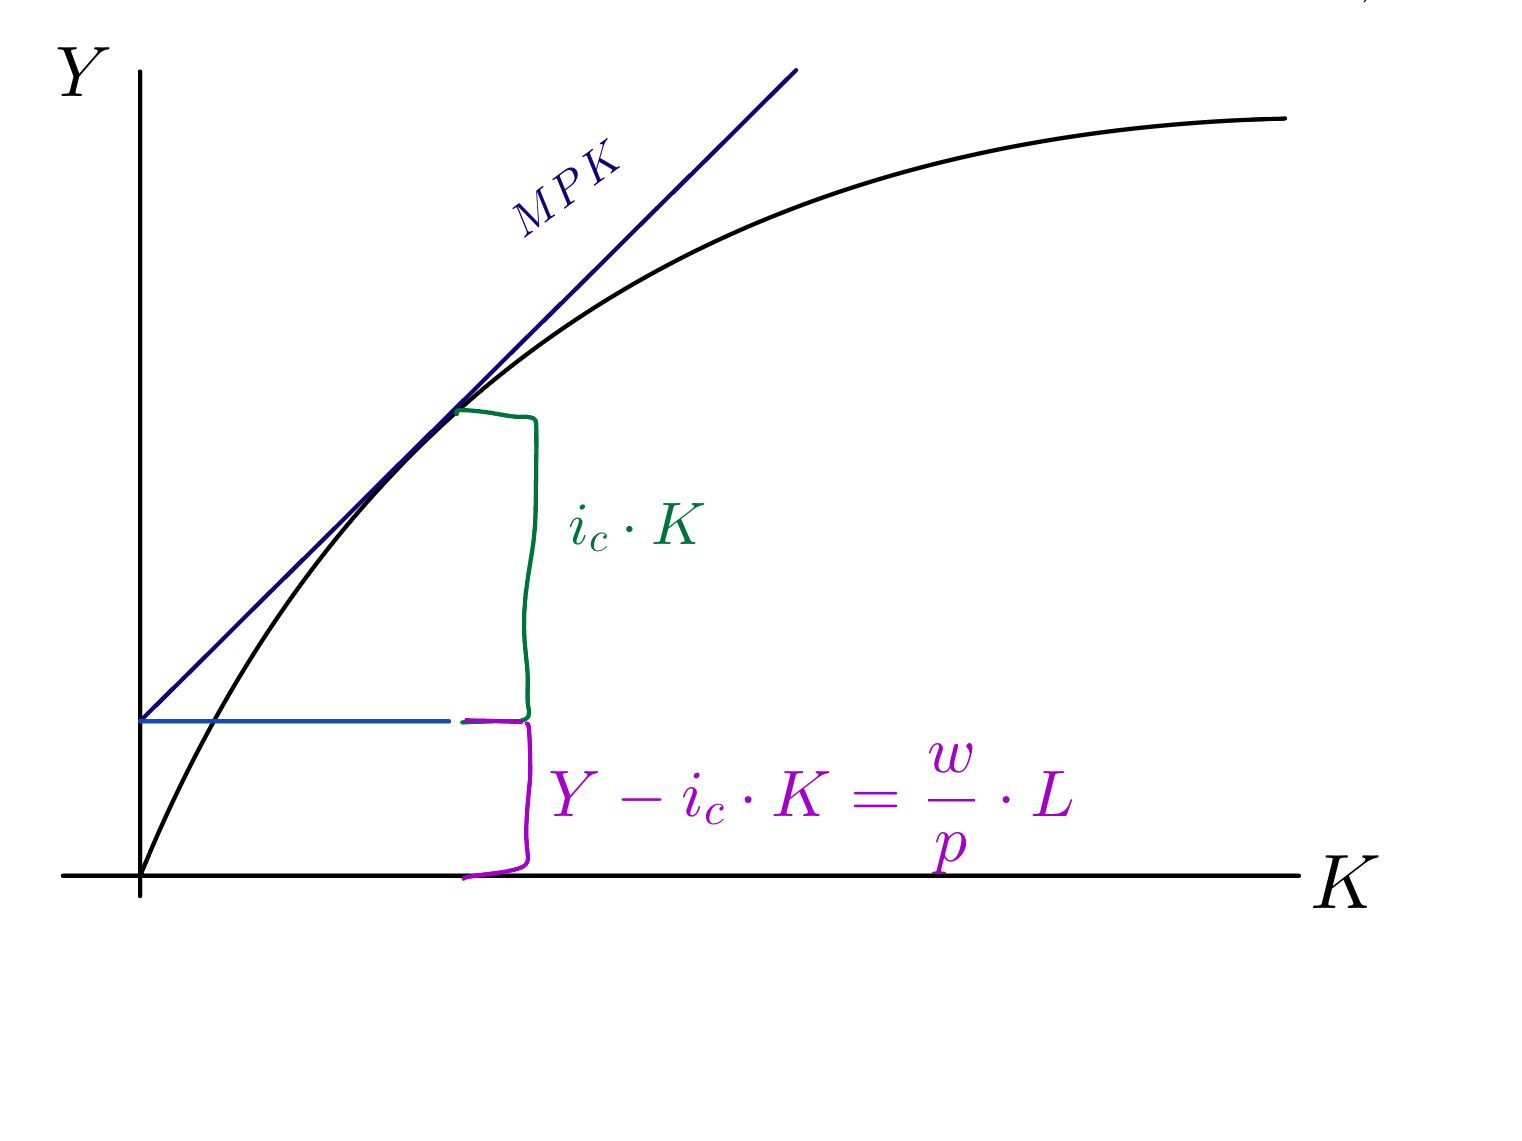
\includegraphics[width=1.1\textwidth]{WhatsApp Image 2024-02-10 at 23.50.58.jpeg}
                \end{center}
                \caption{}
                \label{fig:}
            \end{small}
        \end{figure}
        
    \end{frame}

    \section{פונקציית קוב דאגלס}
    \begin{frame}[allowframebreaks]
        \frametitle{פונקציית קוב דאגלס}
        \begin{equation*}
            Y = AF(K,L) = K^{\a} L^{\beta}
        \end{equation*}

        \begin{equation*}
            Y(\lambda) = AF(\lambda K, \lambda L) = (\lambda K ) ^ \alpha (\lambda L) ^ \beta = \lambda ^ {\alpha + \beta} \cdot K ^ \alpha \cdot L ^ \beta = \lambda ^{\alpha + \beta} Y
        \end{equation*}
        
        \begin{block}{תשואה לגודל}
            \begin{enumerate}
                \item $\alpha + \beta > 1 $ -  תשואה עולה לגודל
                \item $\alpha + \beta = 1 $ -  תשואה קבועה לגודל
                \item $\alpha + \beta < 1 $ -  תשואה יורדת לגודל
            \end{enumerate}
        \end{block}
    
        \framebreak

        \begin{block}{חלקים יחסיים בקוב דאגלס}
            $$S_K = \frac{MPK \cdot K}{Y} = \frac{\alpha \cdot A \cdot K^{\alpha - 1} \cdot L^\beta \cdot K}{AK^\alpha L^\beta} = \alpha$$
            $$S_L = \frac{MPL \cdot L}{Y} = \frac{\beta \cdot A \cdot K^{\alpha} \cdot L^{\beta - 1 } \cdot L }{AK^\alpha L^\beta} = \beta$$
        \end{block}

    \end{frame}


    \section{התחלקות התוצר בשימושים}
    \begin{frame}[allowframebreaks]
        \frametitle{התחלקות התוצר בשימושים}
        \begin{block}{לפי דוח מקו''ש}
        $$\bar Y = C(\bar Y - T) + G_0 + I(r)$$  
        אפשר לראות שהמשתנה האנדוגני היחיד הוא הריבית, שבעזרתו הביקוש מתאים את עצמו לתוצר.      
        \end{block}
        הבהרה : הסוגריים זה לא כפל, הכוונה בפונקציה של מה, לדוגמה צריכה היא פונקציה של מיסים ותוצר.
        
        \begin{block}{שוק ההון}
            הריבית נקבעת בשוק ההון $I = S$
            \begin{enumerate}
                \item כאשר $I > S$ היצע החיסכון במשק נמוך מהביקוש להשקעות, לכן הריבית תעלה עד שהתקיים $I = S$
                \item כאשר $I < S$ היצע החיסכון במשק גדול יותר מהביקוש להשקעות , לכן הריבית תרד עד שהתקיים $I = S$
            \end{enumerate}
        \end{block}

        \framebreak
        \begin{block}{תזכורת}
            $$S_p = Y - T - C$$
            $$S_G = T - G$$
            $$S = S_p + S_G = Y - T - C + T - G = Y - C - G = I$$
        \end{block}
        \begin{figure}
            \begin{small}
                \begin{center}
                    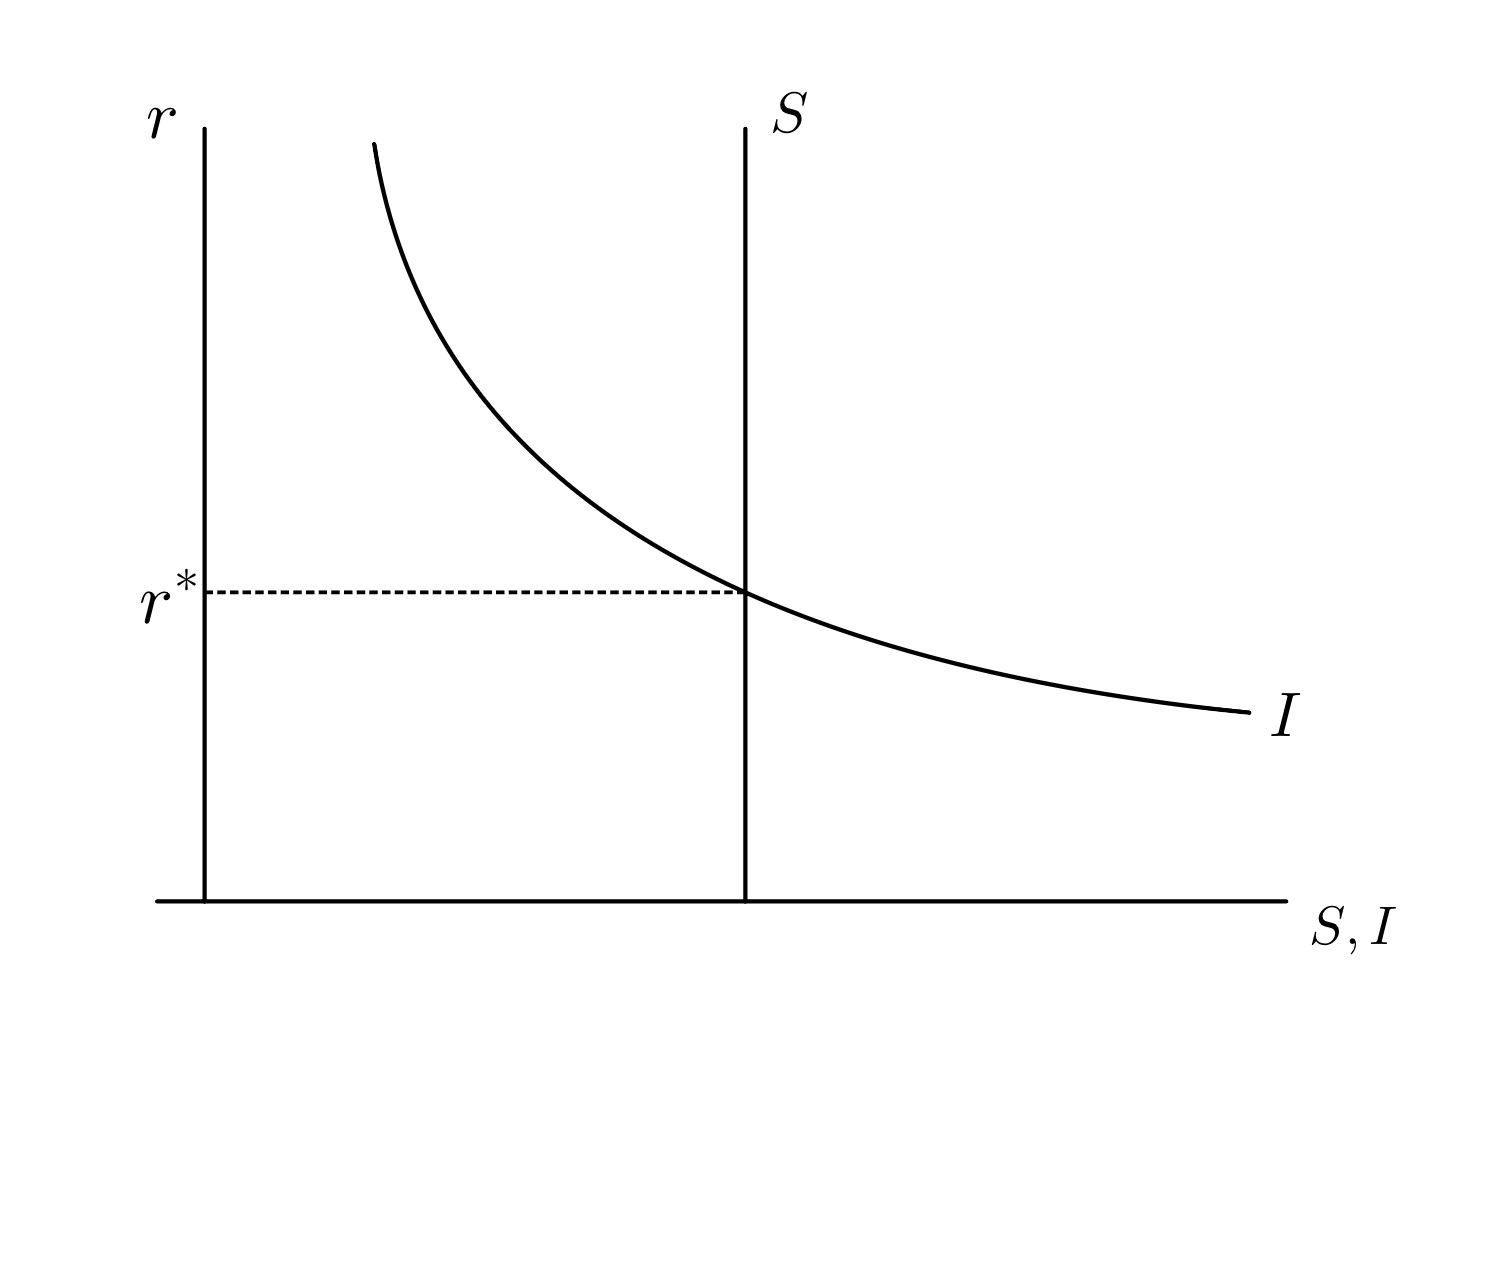
\includegraphics[width=0.95\textwidth]{WhatsApp Image 2024-02-10 at 23.34.52.jpeg}
                \end{center}
                \caption{}
                \label{fig:}
            \end{small}
        \end{figure}
        
    
    \end{frame}
\end{RTL}
\end{document}